\documentclass[tikz,border=6pt]{standalone}
\usetikzlibrary{calc}

\definecolor{SphereOrange}{RGB}{242,171,40}

\tikzset{
  sphere/.style={shade, ball color=SphereOrange, draw=none},
}

\begin{document}
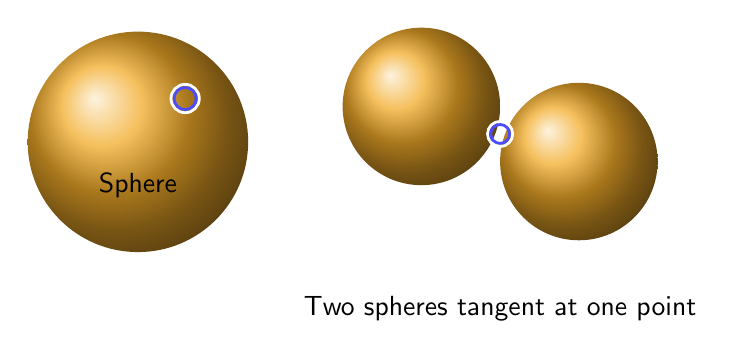
\begin{tikzpicture}[font=\sffamily]

  % --- (A) Single sphere ---
  \begin{scope}
    \coordinate (C) at (0,0);
    \def\r{1.4}
    \path[sphere] (C) circle (\r);

    % optional highlight ring (to mark a point)
    \coordinate (P) at ($(C)+(0.6,0.55)$);
    \draw[white, line width=1.0pt] (P) circle (0.18);
    \draw[blue!70, line width=1.0pt] (P) circle (0.14);

    \node[below=8pt] at (C) {Sphere};
  \end{scope}

  % --- (B) Two spheres touching at one point ---
  \begin{scope}[xshift=4.6cm]
    \def\r{1.0}

    % Centers chosen so the spheres are tangent: distance = 2r
    \coordinate (C1) at (-1.0,0.45);
    \coordinate (C2) at ( 1.0,-0.25);

    % Touch point lies on the segment C1--C2 at distance r from either center
    \coordinate (T) at ($(C1)!0.5!(C2)$);

    \path[sphere] (C1) circle (\r);
    \path[sphere] (C2) circle (\r);

    % mark the touching point
    \draw[white, line width=1.0pt] (T) circle (0.16);
    \draw[blue!70, line width=1.0pt] (T) circle (0.12);

    \node[below=8pt] at (0,-1.55) {Two spheres tangent at one point};
  \end{scope}

\end{tikzpicture}
\end{document}
